\documentclass{article}
\usepackage[utf8]{inputenc}
\usepackage{amsmath}
\usepackage{amsfonts}
\usepackage{enumitem}
\usepackage{amssymb} 
\usepackage{xcolor}
\usepackage{soul}
\usepackage{todonotes}
\usepackage[margin=2.5cm]{geometry}
\graphicspath{ {./images/} }

\title{Probability Theory}
\author{Jin Long Cao, Ethelia Choi}
\date{October 2022}

\begin{document}
\maketitle
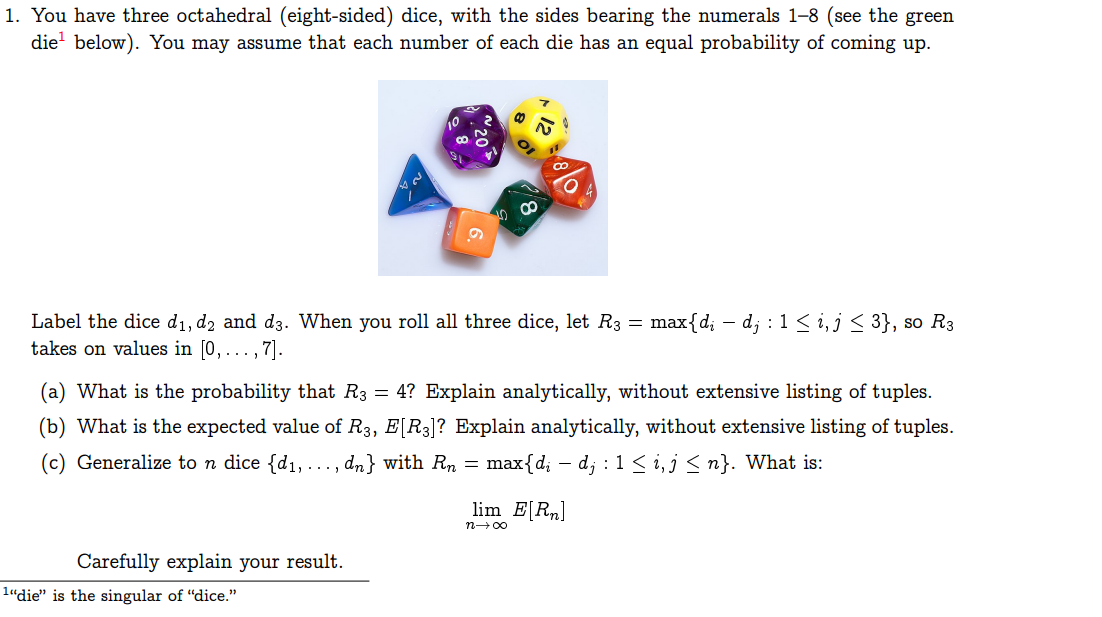
\includegraphics[width=\textwidth]{Probability Theory}

\newpage
\section*{Solutions}
\subsubsection*{(a)} 
% The possible combination that results $R_3=4$ is when
% \begin{enumerate}
%     \item two arbitrary dices are 8 and 4 then the last die $d \in \{4,5,6,7,8\}$
%     \item two arbitrary dices are 7 and 3 then the last die $d \in \{3,4,5,6,7\}$
%     \item two arbitrary dices are 6 and 2 then the last die $d \in \{2,3,4,5,6\}$
%     \item two arbitrary dices are 5 and 1 then the last die $d \in \{1,2,3,4,5\}$
% \end{enumerate}
% with the two arbitrary dice possible being $d_1d_2, d_2d_1, d_2d_3, d_3d_2, d_3d_1,d_1d_3$.\\
% As a demonstration for the fourth possibility, 
% \begin{center}
% \begin{tabular}{||c c c c||} 
%  \hline
%  $d_1$ & $d_2$ & $d_3$ &\\ [0.5ex] 
%  \hline\hline
%  1 & 5 & $x$ & $x \in \{1,2,3,4,5\}$ \\ 
%  \hline
%  1 & $x$ & 5 & repeated rolls: $(d_1,d_2,d_3) = (1,5,5)$ \\
%  \hline
%  $x$ & 1 & 5 & repeated rolls: $(1,1,5)$ \\
%  \hline
%  5 & 1 & $x$ & repeated rolls: $(5,1,5)$ \\
%  \hline 
%  5 & $x$ & 1 & repeated rolls: $(5,1,1)$ \\
%  \hline
%  $x$ & 5 & 1 & repeated rolls: $(5,5,1)$ and $(1,5,1)$\\
%  \hline
% \end{tabular}
% \end{center}
% The repeated rolls are to make sure we don't double count (i.e. $(d_1,d_2,d_3) = (1,5,5)$ is already counted once in the first row, so we don't count it again in the second row). So we have 6 position the dices can be at ($d_1d_2, d_2d_1, d_2d_3, d_3d_2, d_3d_1,d_1d_3$), 4 ways to subtract two dice to make 4, and $5-1=4$ possible values the last die can take (without repeated values). 


We claim that $$P(R_3=4)=\frac{4(6\times 3+ 3\times 2)}{8^3}=\frac{96}{512}=18.75$$
First of all, we have 4 because there are 4 possible pairs of numbers such that $R_3=4$. Namely, $(1, 5), (2, 6), (3, 7), (4, 8)$. Then, for a fixed pair, for example, $(2, 6)$, suppose the first die is 2 and the second die is 6. We are left with two cases for the third die. 
\begin{itemize}
    \item Case 1: The third die is not 2 nor 6.\\
    Then the value of the third die has to be a number between 2 and 6, that is one of $\{3, 4, 5\}$. This is because if the third die is a number bigger than 6 or smaller than 2, $R_3 > 4$. So there are 3 choices for the third die. There are 6 permutations of these 3 distinct numbers. For example, if the third die is 3, the permutations are $(2, 3, 4), (2, 4, 3), (3, 2, 4), (3, 4, 2), (4, 2, 3), (4, 3, 2)$. Thus, this gives us $6\times 3$.
    \item Case 2: The third die is 2 or 6.\\
    So there are 2 choices for the third die. This time, we will only have 3 permutations because two of the three elements are the same. We can also think of this as double counting where we divide the 6 permutations by 2, which also gives us 3. For example, suppose the third die is 2, then $(2, 2, 6), (2, 6, 2), (6, 2, 2)$.  Thus, we arrive at $3\times 2$.
\end{itemize}
One of these 2 cases must happen so we add these two, which is $6\times 3+3\times 2$. Then, we have 4 pairs, so we multiply and get $4(6\times 3+3\times 2)$. Then the total probability is $8^3$ because there are 3 dice and each die can take 8 different numbers. We divide the product by the total probability because that tells us of all 512 different possible combinations we can get rolling 3 dices, 96 of those will satisfy the requirement $R_3=4$. 


% 8-4	but not if third dice is 1,2,3
% 7-3	but not if third dice is 1,2,8
% 6-2	but not if third dice is 1,7,8
% 5-1	but not if third dice is 6,7,8
% d_1   d_2     d_3 \\
% 1     5       x   $x \in \{1,2,3,4,5\}$ \\
% 1     x       5   Repeats 155\\
% x     1       5   Repeats 115\\
% 5	    1	    x   Repeats 515\\
% x 	5      	1   Repeats 151\\
% 5	    x   	1   Repeats 551, 511\\
\subsubsection*{(b)} 
% Expectation of maximum:
% https://www.quora.com/How-do-you-find-the-expected-value-of-the-maximum-of-n-discrete-i-i-d-random-variables

We propose that $$E[R_3]=\sum_{i=0}^7 i\times \frac{(8-i)(6\times (i-1)+3\times 2)}{8^3}$$ Substituting $i=0,1,\dots, 7$ and calculating the sum, we have that $E[R_3] = 3.9375$. 
In the sum, $i$ is just the value of $R_3$ while the fraction represents $P(R_3)=i$. \\~\\
Now we look into the fraction. We have $(8-i)$ because there are $(8-i)$ ways of subtracting two dice to make $i$. We arrived at this by substituting different $k$ for $R_3=k$ and found a pattern. That is, 
\begin{itemize}
    \item Let $k=0$, then this means both dice have to roll the same element. Since there are 8 distinct numbers, there are 8 possible pairs.
    \item Let $k=1$, then the combinations are $(1,2), (2,3), \dots, (7,8)$. There are 7 possible pairs. 
    \item Let $k=2$, then the combinations are $(1,3), (2,4), \dots, (6,8)$. There are 6 possible pairs. 
    \item \dots
    \item Let $k=7$, then the only combination is $(1, 8)$. There is only 1 possible pair.
\end{itemize}
Then, for a fixed pair $(a, b)$, suppose for the first dice, we rolled $a$, and for the second dice, we rolled $b$. This leaves us with the third dice. Suppose for the third dice we rolled $c$. There are two different scenarios that can happen:
\begin{itemize}
    \item Case 1: $c\neq a$ and $c\neq b$. \\ 
    Notice that $c$ has to be a number between $a$ and $b$, otherwise, $R_3$ will be greater than the value it should be. This gives us $i-1$ choices for $c$. Next, there are 6 permutations to order these 3 distinct elements: $(a, b, c), (a, c, b), (b, a, c), (b, c, a), (c, a, b), (c, b, a)$. So this gives us $6\times (i-1)$. 
    \item Case 2: $c=a$ or $c=b$.\\
    There are 2 choices for $c$. Then notice that since one element is repeated, we need to account for double counting by dividing the number of permutations, 6, by 2. (Double counting means $(a, b, c) = (a, c, b)$ if $b=c$.) Thus, there are 3 permutations for this case. This gives us $3\times 2$.
\end{itemize}
Now we put everything together. Since for every fixed pair, one of the two cases can happen, we add the two possibilities, which is $6\times (i-1)+3\times 2$. 
Next, since we have $(8-i)$ different pairs, we multiply $6\times (i-1)+3\times 2$ by $(8-i)$. This gives us $(8-i)(6\times (i-1)+3\times 2)$, which is what we have in the numerator. Lastly, we divide the product by $8^3$ because we have 3 dice and each can take 8 different values. 


\subsubsection*{(c)}
First of all, notice that 
\begin{align*}
    \lim_{n\to\infty} (E[R_n])&=\lim_{n\to\infty}\bigg(\sum_{i=0}^7 i\cdot P(R_n=i)\bigg)\\
    &=\sum_{i=0}^7 \bigg(\lim_{n\to\infty} i\cdot P(R_n=i)\bigg)\\
    &=\sum_{i=0}^7 i\cdot \bigg(\lim_{n\to\infty} P(R_n=i)\bigg)\tag{since $i$ is a constant to the limit}\\
    &= 0\cdot \bigg(\lim_{n\to\infty} P(R_n=0)\bigg)+1\cdot\bigg(\lim_{n\to\infty} P(R_n=1)\bigg) +\dots+7\cdot \bigg(\lim_{n\to\infty} P(R_n=7)\bigg)
\end{align*}
Now we will look into each $P(R_n=k)$ for all $k$ from 0 to 7 when $n$ approaches infinity. Here, it is important to note that each number of each die has an equal probability of coming up. \\~\\
\underline{How can we have $R_n=0$ when $n$ is large?}\\
This means 2 of our $n$ rolls need to be identical. Since we have 8 distinct numbers, when we roll $n$ dices, it is highly likely that we will have at least 2 rolls that give the same number. In fact, if we think about it, the probability of this happening is close to 1. However, if $R_n=0$, this means the remaining $n-2$ dice rolls will also have to land on the same number. Or else, if at least one dice roll is one of the other 7 numbers, then the max difference, $R_n$ will be greater than 0. In other words, once we rolled the first die, for the remaining $n-1$ dice rolls, we need to avoid 7 numbers. We can see that the probability of this happening is close to 0 when $n$ is large, i.e. $\lim_{n\to\infty} P(R_n=0)=0$.\\~\\
\underline{How can we have $R_n=1$ when $n$ is large?}\\
We need 2 rolls to be one of the following 7 pairs: $(1,2), (2,3),\dots, (7,8)$. Suppose for dice $i$ we rolled 1 and for dice $j$ we rolled 2, where $i, j\in [1, n]$. Then, the other $n-2$ dice rolls will have to be either 1 or 2. Otherwise, if we rolled any other number from 3 to 7, $R_n$ will be greater than 1. Notice that if we picked a different pair for dice $i$ and $j$, the same issue will arise. So in other words, after we have fixed two distinct numbers that has a difference of 1, for every roll we make onwards, we need to avoid 6 numbers. Again, this is nearly impossible when $n$ is large. Thus, $\lim_{n\to\infty} P(R_n=1)=0$.\\~\\
 Now, we will look at when $k=6$. \\~\\
\underline{How can we have $R_n=6$ when $n$ is large?} \\
We need 2 rolls to be one of the following 2 pairs: $(1,7), (2,8)$. Suppose of all $n$ dice, we rolled at least one 1 and one 7. We can see the probability of this happening is extremely high because $n$ is large. Then, for the max difference to be 6, for the remaining $n-2$ rolls, we cannot roll an 8. Similarly, if our pair was $(2, 8)$, we will have to avoid rolling 1. In other words, we have to avoid one number. However, since $n$ is arbitrarily large, the chances of never rolling one number is extremely small. Thus, $\lim_{n\to\infty} P(R_n=6)=0$. \\~\\
Therefore, we can generalize the above cases and see that when we want $R_n=k$, for every $n-2$ dice roll, we will need to avoid rolling $(7-k)$ numbers. So we can repeat this analysis for $k = 3, 4, 5$ and we will arrive at the same result, that $\lim_{n\to\infty} P(R_n=k)=0$ for all $k\in [0, 6]$.\\~\\
\underline{How can we have $R_n=7$ when $n$ is large?}\\
Using our observation, we know that we need to avoid $(7-7)=0$ numbers. We will see in a bit whether this is true. Since we roll so many dices, it is guaranteed that we will roll at least one 1 and one 8. Notice that this is the only pair that gives a difference of 7. Then it does not matter what we roll for the remaining $n-2$ dices, $R_n$ will be equal to 7. So indeed, we need to avoid 0 numbers. Since there are no restrictions, $\lim_{n\to\infty}P(R_n=7)=1$. 
\\~\\
Therefore, 
\begin{align*}
    \lim_{n\to\infty} (E[R_n])&=0\cdot \bigg(\lim_{n\to\infty} P(R_n=0)\bigg)+1\cdot\bigg(\lim_{n\to\infty} P(R_n=1)\bigg) +\dots+7\cdot \bigg(\lim_{n\to\infty} P(R_n=7)\bigg)\\
    &= 0\cdot 0+1\cdot 0+ \dots+6\cdot 0+7\cdot 1\\
    &= 7
\end{align*}
\end{document}
